\documentclass[12pt]{article}\usepackage[]{graphicx}\usepackage[]{color}
%% maxwidth is the original width if it is less than linewidth
%% otherwise use linewidth (to make sure the graphics do not exceed the margin)
\makeatletter
\def\maxwidth{ %
  \ifdim\Gin@nat@width>\linewidth
    \linewidth
  \else
    \Gin@nat@width
  \fi
}
\makeatother

\definecolor{fgcolor}{rgb}{0.345, 0.345, 0.345}
\newcommand{\hlnum}[1]{\textcolor[rgb]{0.686,0.059,0.569}{#1}}%
\newcommand{\hlstr}[1]{\textcolor[rgb]{0.192,0.494,0.8}{#1}}%
\newcommand{\hlcom}[1]{\textcolor[rgb]{0.678,0.584,0.686}{\textit{#1}}}%
\newcommand{\hlopt}[1]{\textcolor[rgb]{0,0,0}{#1}}%
\newcommand{\hlstd}[1]{\textcolor[rgb]{0.345,0.345,0.345}{#1}}%
\newcommand{\hlkwa}[1]{\textcolor[rgb]{0.161,0.373,0.58}{\textbf{#1}}}%
\newcommand{\hlkwb}[1]{\textcolor[rgb]{0.69,0.353,0.396}{#1}}%
\newcommand{\hlkwc}[1]{\textcolor[rgb]{0.333,0.667,0.333}{#1}}%
\newcommand{\hlkwd}[1]{\textcolor[rgb]{0.737,0.353,0.396}{\textbf{#1}}}%
\let\hlipl\hlkwb

\usepackage{framed}
\makeatletter
\newenvironment{kframe}{%
 \def\at@end@of@kframe{}%
 \ifinner\ifhmode%
  \def\at@end@of@kframe{\end{minipage}}%
  \begin{minipage}{\columnwidth}%
 \fi\fi%
 \def\FrameCommand##1{\hskip\@totalleftmargin \hskip-\fboxsep
 \colorbox{shadecolor}{##1}\hskip-\fboxsep
     % There is no \\@totalrightmargin, so:
     \hskip-\linewidth \hskip-\@totalleftmargin \hskip\columnwidth}%
 \MakeFramed {\advance\hsize-\width
   \@totalleftmargin\z@ \linewidth\hsize
   \@setminipage}}%
 {\par\unskip\endMakeFramed%
 \at@end@of@kframe}
\makeatother

\definecolor{shadecolor}{rgb}{.97, .97, .97}
\definecolor{messagecolor}{rgb}{0, 0, 0}
\definecolor{warningcolor}{rgb}{1, 0, 1}
\definecolor{errorcolor}{rgb}{1, 0, 0}
\newenvironment{knitrout}{}{} % an empty environment to be redefined in TeX

\usepackage{alltt}
 
\usepackage[margin=1in]{geometry}
\usepackage{amsmath,amsthm,amssymb, mathtools}
\usepackage[T1]{fontenc}
\usepackage{lmodern}
\usepackage{fixltx2e}
\usepackage[shortlabels]{enumitem}
 
\newcommand{\N}{\mathbb{N}}
\newcommand{\R}{\mathbb{R}}
\newcommand{\Z}{\mathbb{Z}}
\newcommand{\Q}{\mathbb{Q}}
 
\newenvironment{theorem}[2][Theorem]{\begin{trivlist}
\item[\hskip \labelsep {\bfseries #1}\hskip \labelsep {\bfseries #2.}]}{\end{trivlist}}
\newenvironment{lemma}[2][Lemma]{\begin{trivlist}
\item[\hskip \labelsep {\bfseries #1}\hskip \labelsep {\bfseries #2.}]}{\end{trivlist}}
\newenvironment{exercise}[2][Exercise]{\begin{trivlist}
\item[\hskip \labelsep {\bfseries #1}\hskip \labelsep {\bfseries #2.}]}{\end{trivlist}}
\newenvironment{problem}[2][Problem]{\begin{trivlist}
\item[\hskip \labelsep {\bfseries #1}\hskip \labelsep {\bfseries #2.}]}{\end{trivlist}}
\newenvironment{question}[2][Question]{\begin{trivlist}
\item[\hskip \labelsep {\bfseries #1}\hskip \labelsep {\bfseries #2.}]}{\end{trivlist}}
\newenvironment{corollary}[2][Corollary]{\begin{trivlist}
\item[\hskip \labelsep {\bfseries #1}\hskip \labelsep {\bfseries #2.}]}{\end{trivlist}}
\newcommand{\textfrac}[2]{\dfrac{\text{#1}}{\text{#2}}}
\IfFileExists{upquote.sty}{\usepackage{upquote}}{}
\begin{document}

\title{Statistical Rethinking: Chapter 5 - Multivariate Linear Models}

\author{Chris Hayduk}
\date{\today}

\maketitle




\section{Easy}

\begin{problem}{5E1}
\text{ }\\
Which of the linear models below are multiple linear regressions?
\begin{enumerate}
	\item $\mu$\textsubscript{i} = $\alpha$ + $\beta$x\textsubscript{i}
	\item $\mu$\textsubscript{i} = $\beta$\textsubscript{x}x\textsubscript{i} + $\beta$\textsubscript{z}z\textsubscript{i}
	\item $\mu$\textsubscript{i} = $\alpha$ + $\beta$(x\textsubscript{i} - z\textsubscript{i})
	\item $\mu$\textsubscript{i} = $\alpha$ + $\beta$\textsubscript{x}x\textsubscript{i} + $\beta$\textsubscript{z}z\textsubscript{i}
\end{enumerate}
\end{problem}

Linear models 2 and 4 are multiple linear regressions.

\begin{problem}{5E2}
\text{ }\\
Write down a multiple regression to evaluate the claim: \textit{Animal diversity is linearly related to latitude, but only after controlling for plant diversity.} You just need to write down the model definition.
\end{problem}

\begin{center}
animal diversity\textsubscript{i} $\sim$ Normal($\mu$\textsubscript{i}, $\sigma$)\\
$\mu$\textsubscript{i} = $\beta$\textsubscript{latitude}latitude\textsubscript{i} + $\beta$\textsubscript{diversity}diversity\textsubscript{i}\\
$\beta$\textsubscript{latitude} $\sim$ Normal(0, 10)\\
$\beta$\textsubscript{diversity} $\sim$ Normal(0, 10)\\
$\sigma$ $\sim$ Uniform(0, 10)
\end{center}

\begin{problem}{5E3}
\text{ }\\
Write down a multiple regression to evaluate the claim: \textit{Neither amount of funding nor size of laboratory is by itself a good predictor of time to PhD degree; but together these variables are both positively associated with time to degree.} Write down the model definition and indicate which side of zero each slope parameter should be on.
\end{problem}

\begin{center}
time\textsubscript{i} $\sim$ Normal($\mu$\textsubscript{i}, $\sigma$)\\
$\mu$\textsubscript{i} = $\beta$\textsubscript{lab size}lab size\textsubscript{i} + $\beta$\textsubscript{funding}funding\textsubscript{i}\\
$\beta$\textsubscript{lab size} $\sim$ Normal(0, 10)\\
$\beta$\textsubscript{funding} $\sim$ Normal(0, 10)\\
$\sigma$ $\sim$ Uniform(0, 10)
\end{center}

Both parameters should have slopes greater than zero since the problem specifies that "together the variables are both positively associated with time to degree".

\begin{problem}{5E4}
\text{ }\\
Suppose you have a single categorical predictor with 4 levels (unique values), labeled A, B, C, and D. Let A\textsubscript{i} be an indicator variable that is 1 where case \textit{i} is in category A. Also suppose B\textsubscript{i}, C\textsubscript{i}, and D\textsubscript{i} for the other categories. Now which of the following linear models are inferentially equivalent ways to include the categorical variable in a regression? Models are inferentially equivalent when it's possible to compute one posterior distribution from the posterior distribution of another model.
\begin{enumerate}
	\item $\mu$\textsubscript{i} = $\alpha$ + $\beta$\textsubscript{A}A\textsubscript{i} + $\beta$\textsubscript{B}B\textsubscript{i} + $\beta$\textsubscript{D}D\textsubscript{i}
	\item $\mu$\textsubscript{i} = $\alpha$ + $\beta$\textsubscript{A}A\textsubscript{i} + $\beta$\textsubscript{B}B\textsubscript{i} + $\beta$\textsubscript{C}C\textsubscript{i} + $\beta$\textsubscript{D}D\textsubscript{i}
	\item $\mu$\textsubscript{i} = $\alpha$ + $\beta$\textsubscript{B}B\textsubscript{i} + $\beta$\textsubscript{C}C\textsubscript{i} + $\beta$\textsubscript{D}D\textsubscript{i}
	\item $\mu$\textsubscript{i} = $\alpha$\textsubscript{A}A\textsubscript{i} + $\alpha$\textsubscript{B}B\textsubscript{i} + $\alpha$\textsubscript{C}C\textsubscript{i} + $\alpha$\textsubscript{D}D\textsubscript{i}
	\item $\mu$\textsubscript{i} = $\alpha$\textsubscript{i}(1 - B\textsubscript{i} - C\textsubscript{i} - D\textsubscript{i}) + $\alpha$\textsubscript{B}B\textsubscript{i} + $\alpha$\textsubscript{C}C\textsubscript{i} + $\alpha$\textsubscript{D}D\textsubscript{i}
\end{enumerate}
\end{problem}

Models 1, 3, 4, and 5 are all inferentially equivalent.

\section{Medium}

\begin{problem}{5M1}
\text{ }\\
Invent your own example of a spurious correlation. An outcome variable should be correlated with both predictor variables. But when both predictors are entered in the same model, the correlation between the outcome and one of the predictors should mostly vanish (or at least be greatly reduced).
\end{problem}

\begin{knitrout}
\definecolor{shadecolor}{rgb}{0.969, 0.969, 0.969}\color{fgcolor}\begin{kframe}
\begin{alltt}
\hlstd{N} \hlkwb{<-} \hlnum{1e4}
\hlstd{x.real} \hlkwb{<-} \hlkwd{rnorm}\hlstd{(}\hlkwc{n} \hlstd{= N,} \hlkwc{mean} \hlstd{=} \hlnum{1}\hlstd{,} \hlkwc{sd} \hlstd{=} \hlnum{1}\hlstd{)}
\hlstd{x.spurious} \hlkwb{<-} \hlkwd{rnorm}\hlstd{(}\hlkwc{n} \hlstd{= N,} \hlkwc{mean} \hlstd{= x.real)}
\hlstd{y} \hlkwb{<-} \hlkwd{rnorm}\hlstd{(}\hlkwc{n} \hlstd{= N,} \hlkwc{mean} \hlstd{= x.real)}

\hlstd{df} \hlkwb{<-} \hlkwd{data.frame}\hlstd{(}\hlkwc{y} \hlstd{= y,} \hlkwc{x.real} \hlstd{= x.real,} \hlkwc{x.spurious} \hlstd{= x.spurious)}
\hlkwd{pairs}\hlstd{(df)}
\end{alltt}
\end{kframe}
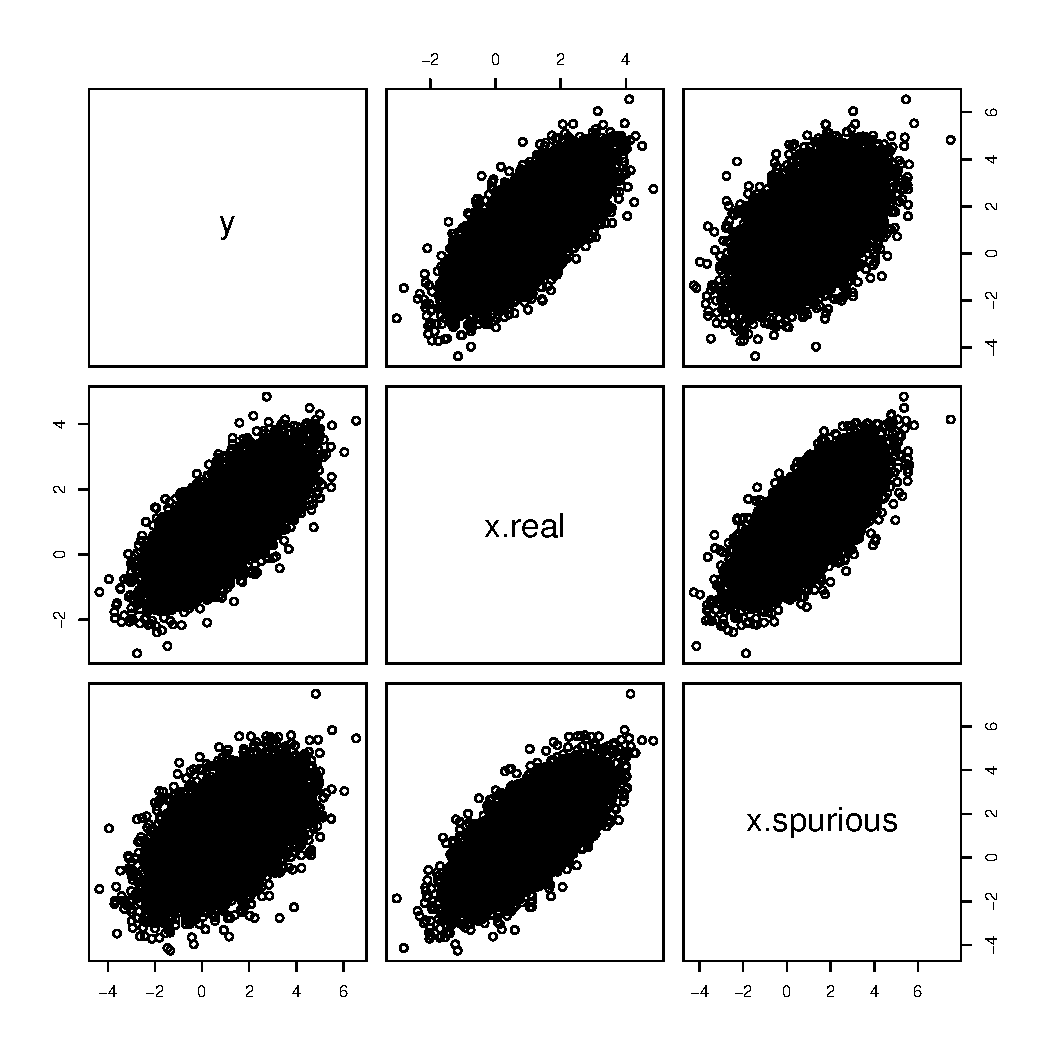
\includegraphics[width=\maxwidth]{figure/unnamed-chunk-2-1} 
\begin{kframe}\begin{alltt}
\hlstd{model} \hlkwb{<-} \hlkwd{lm}\hlstd{(y} \hlopt{~} \hlstd{x.real} \hlopt{+} \hlstd{x.spurious)}
\hlkwd{precis}\hlstd{(model)}
\end{alltt}
\begin{verbatim}
##              Mean StdDev  5.5% 94.5%
## (Intercept)  0.02   0.01 -0.01  0.04
## x.real       1.01   0.01  0.99  1.03
## x.spurious  -0.01   0.01 -0.03  0.01
\end{verbatim}
\end{kframe}
\end{knitrout}

\begin{problem}{5M2}
\text{ }\\
Invent your own example of a masked relationship. An outcome variable should be correlated with both predictor variables, but in opposite directions. And the two predictor variables should be correlated with one another.
\end{problem}

\begin{knitrout}
\definecolor{shadecolor}{rgb}{0.969, 0.969, 0.969}\color{fgcolor}\begin{kframe}
\begin{alltt}
\hlstd{N} \hlkwb{<-} \hlnum{1e4}
\hlstd{rho} \hlkwb{<-} \hlnum{0.7}

\hlstd{x.pos} \hlkwb{<-} \hlkwd{rnorm}\hlstd{(N)}
\hlstd{x.neg} \hlkwb{<-} \hlkwd{rnorm}\hlstd{(N, rho}\hlopt{*}\hlstd{x.pos,} \hlkwd{sqrt}\hlstd{(}\hlnum{1}\hlopt{-}\hlstd{rho}\hlopt{^}\hlnum{2}\hlstd{))}
\hlstd{y} \hlkwb{<-} \hlkwd{rnorm}\hlstd{(N, x.pos} \hlopt{-} \hlstd{x.neg)}

\hlstd{df} \hlkwb{<-} \hlkwd{data.frame}\hlstd{(}\hlkwc{y} \hlstd{= y,} \hlkwc{x.pos} \hlstd{= x.pos,} \hlkwc{x.neg} \hlstd{= x.neg)}
\hlkwd{pairs}\hlstd{(df)}
\end{alltt}
\end{kframe}
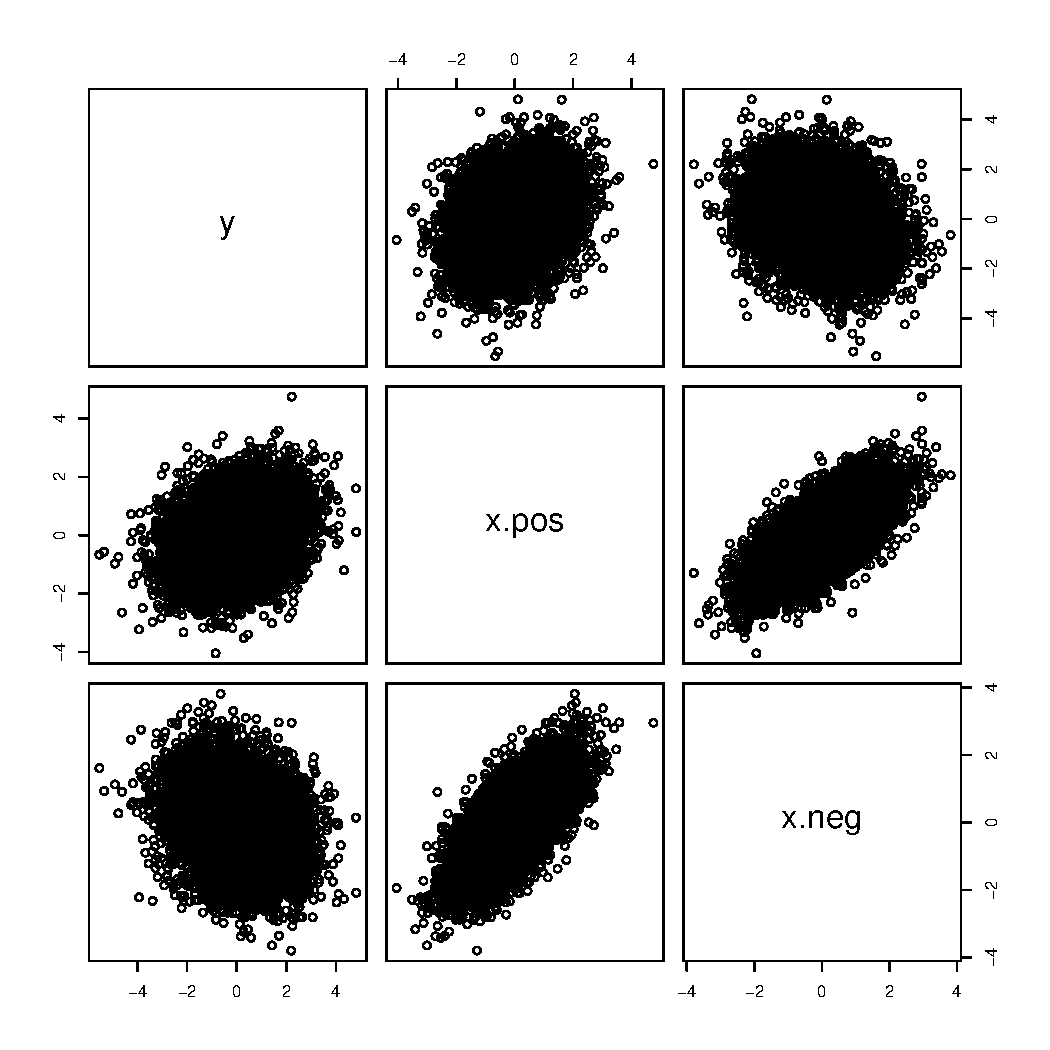
\includegraphics[width=\maxwidth]{figure/unnamed-chunk-3-1} 
\begin{kframe}\begin{alltt}
\hlstd{model} \hlkwb{<-} \hlkwd{lm}\hlstd{(y} \hlopt{~} \hlstd{x.pos} \hlopt{+} \hlstd{x.neg)}
\hlkwd{precis}\hlstd{(model)}
\end{alltt}
\begin{verbatim}
##              Mean StdDev  5.5% 94.5%
## (Intercept)  0.00   0.01 -0.02  0.01
## x.pos        0.99   0.01  0.97  1.01
## x.neg       -1.00   0.01 -1.02 -0.98
\end{verbatim}
\end{kframe}
\end{knitrout}

\begin{problem}{5M3}
\text{ }\\
It is sometimes observed that the best predictor of fire risk is the presence of firefighters - States and localities with many firefighters also have more fires. Presumably firefightes do not \textit{cause} fires. Nevertheless, this is not a spurious correlation. Instead fires cause firefighters. Consider the same reversal of causal inference in the context of the divorice and marriage data. How might a high divorce rate cause a higher marriage rate? Can you think of a way to evaluate this relationship, using multiple regression?
\end{problem}



\end{document}
